%!TEX root = ../proteoform_suite_manual.tex
%---------------------------------------------------------------------
%	IDENTIFIED PROTEOFORMS
%---------------------------------------------------------------------

\section{Identified Proteoforms}


\subsection{Overview}

On this page, all identified proteoforms are displayed, including intact-mass identification (from proteoform family construction) and top-down identifications (from loaded top-down results). The results automatically refresh each time the page is loaded. 

\subsection{Results}
\begin{itemize}
	\item Compare With other Top-Down Results: option to select another top-down hit results file and export and Excel file comparing intact-mass identifications with top-down identifications
	\item Table Filters: filter Identified Intact-Mass Experimental Proteoforms table (top left) and Top-Down Proteoforms table (top right) by any entered text
	\item Identified Intact-Mass Experimental Proteoforms: the left table displays experimental proteoforms identified by intact-mass analysis (proteoform family construction).  See the Aggregated Proteoforms table in the \textbf{Aggregated Proteoforms} section for column descriptions. 
	\begin{figure}[h]
\centering
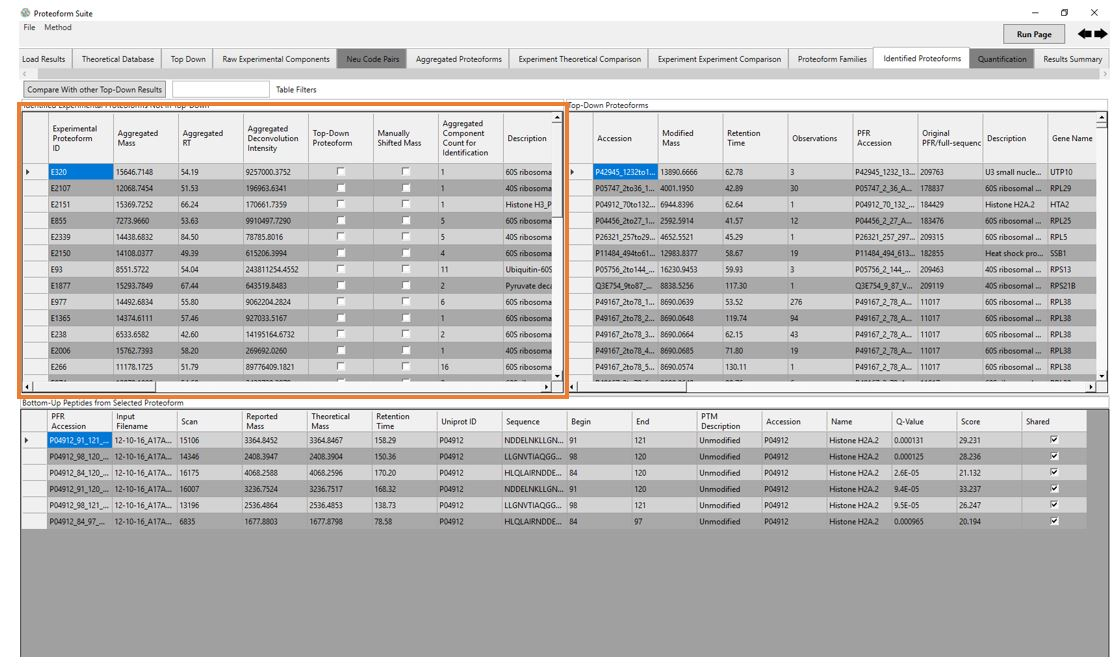
\includegraphics[scale=0.45]{figures/identified1.jpg}
\end{figure}
\pagebreak
\item Top-Down Proteoforms: the right table displays top-down proteoform identifications (aggregated from top-down hit results loaded from top-down results). See the Top-Down Proteoforms table in the \textbf{Top-Down Proteoforms} section for column descriptions.
	\begin{figure}[h]
\centering
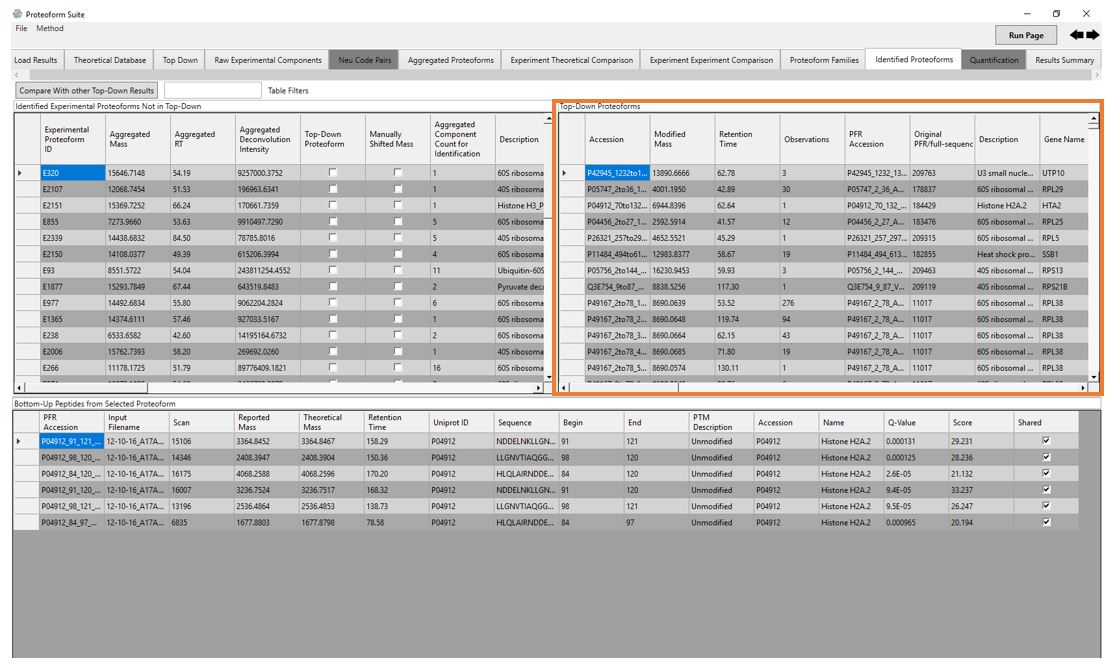
\includegraphics[scale=0.45]{figures/identified2.jpg}
\end{figure}
\item Bottom-Up Peptides from Selected Proteoform: the bottom table displays bottom-up peptides from the selected proteoform in either the Identified Intact-Mass Experimental Proteoforms table or the Top-Down Proteoforms table. See the Bottom-Up Peptides table in the \textbf{Top-Down Proteoforms} section for column descriptions.
	\begin{figure}[h]
\centering
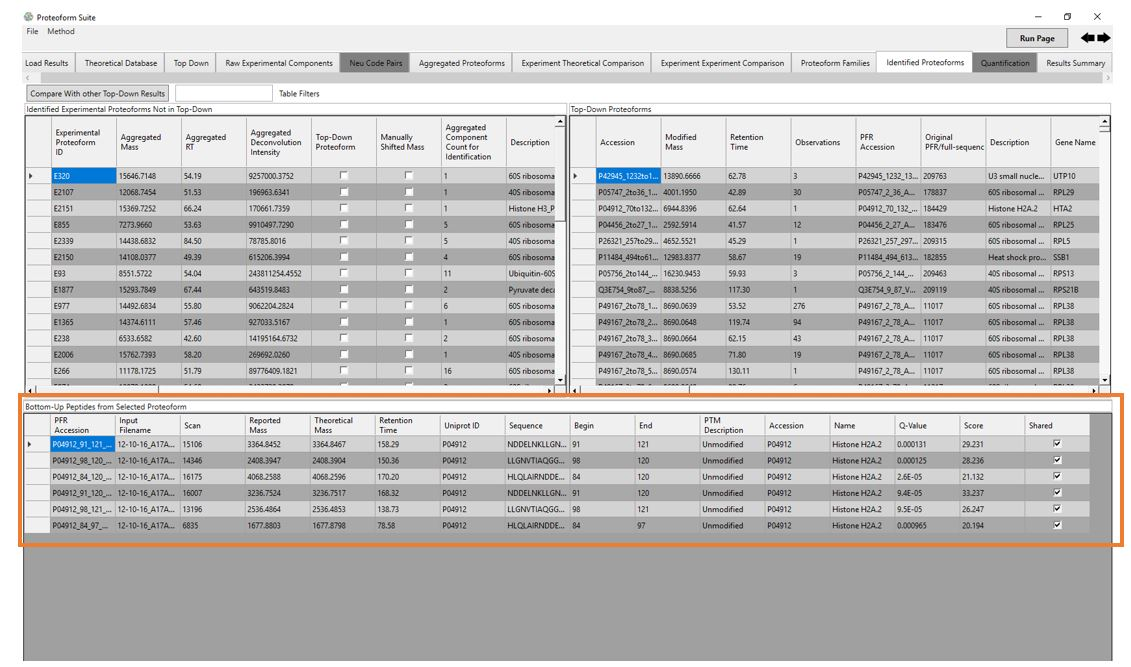
\includegraphics[scale=0.45]{figures/identified3.jpg}
\end{figure}
\end{itemize}